\documentclass{article}
\usepackage[utf8]{inputenc}
\usepackage{amsmath}
\usepackage{graphicx}

\title{Report\\Numerical Simulation of Beam Propagation including Error Convergence Analysis}
\date{15-05-2018}

\author{Prepared by: Nicolae Cadin \\Supervised by: Ramon Springer}

\begin{document}
	
	
	\pagenumbering{gobble}
	\maketitle
	\newpage
	\tableofcontents
	\pagenumbering{arabic}
	
	\newpage
	\section{Introduction}
	Beam propagation in media is of high interest for scientists and also for industrial purposes. 
	In this report beam propagation will be simulated, problems will be discussed. The purpose of the project is to compare numerical method and analytical solution of beam propagation. Convergence of used numerical method is to be shown. For the simplicity simulation of beam propagation is done in free space, linear medium, at zero incident angle, so to fit the scope of mini-project, later on can be extended for more sophisticated cases.
	\subsection{Analytical solution}
	To better analytically understand propagation of beam in space we should solve Helmholz Equation.
	\begin{center}
		$(\nabla^2+k^2)E = 0$		
	\end{center}
	This equation generally holds for electromagnetic wave, hence for electric and magnetic field components, for simplicity we chose electric field $E$. Here $k$ is wave number and is equal to $2\pi n/\lambda$, where $\lambda$ is wavelength, $n$ is refractive index of medium (here we assume it to be equal to 1). As assumption we consider that our wave propagates in $z$ direction and electric field can be represented in next form.
	\begin{center}
		$E(x,y,z)=u(x,y,z)e^{-ik_oz}$
	\end{center}
	$u$ is complex function which describes non-plane part of the beam. Substituting our ansatz into Helmholtz equation in cartesian coordinates and doing some simplifications we get.

	\[\frac{\partial^2 u}{\partial x^2}+ \frac{\partial^2 u}{\partial y^2}+ \frac{\partial^2 u}{\partial z^2} - 2ik_o\frac{\partial u}{\partial z}+(k^2-k_o^2)u=0\]
	Using paraxial approximation we see that third term is smaller than other, therefore can be neglected, as result we get following equation.
	
	\begin{equation}
	\frac{\partial^2 u}{\partial x^2}+ \frac{\partial^2 u}{\partial y^2} - 2ik_o\frac{\partial u}{\partial z}+(k^2-k_o^2)u=0
	\end{equation}
	Solving this differential equation we find $u$ hence we find $E$. We assume that $k = k_o$, therefore solution for one dimensional case, where wave propagates in z-direction and oscillates in xz plane is,
	
	\[E(x,z)=E_o\bigg(\frac{w_o}{w(z)}\bigg)^{\frac{1}{2}}exp\bigg(\frac{x^2}{w(z)^2}\bigg)exp\bigg(-i\Big(k_oz+k_o\frac{x^2}{2R(z)}-\phi(z)\Big)\bigg)\]
	where $w(z)$ is beam radius, $w_o = w(0)$ is beam waist, $E_o$ is electric field amplitude, $R(z)$ is beam curvature, $\phi$ is Gouy phase. Their explicit mathematical formula can be found in the table below. This electric field formula will be later used as reference to numerical solution.
	Intensity can be calculated based on electric field, $I = \frac{\epsilon _o c n_o}{2}|E_z|^2$.
	
%	\[w(z)= w_o\sqrt{1+\Big(\frac{z\lambda}{\pi w_o^2}\Big)^2}\]
%	\[R=z\bigg[1+\Big(\frac{\pi w_o^2}{z\lambda}\Big)^2\bigg]\]
%	\[\phi(z)=arctan\Big(\frac{z\lambda}{\pi w_o^2}\Big)\]

	\begin{table}[h!]
		\begin{center}
%			\caption{Values.}
			\label{tab:table1}
			\begin{tabular}{c| c| c} % <-- Alignments: 1st column left, 2nd middle and 3rd right, with vertical lines in between
				\textbf{Beam Radius} & \textbf{Beam Curvature} & \textbf{Gouy phase}\\
				\hline
				&&\\
				$w(z)= w_o\sqrt{1+\Big(\frac{z\lambda}{\pi w_o^2}\Big)^2}$ & $R=z\bigg[1+\Big(\frac{\pi w_o^2}{z\lambda}\Big)^2\bigg]$ & $\phi(z)=arctan\Big(\frac{z\lambda}{\pi w_o^2}\Big)$\\
			\end{tabular}
		\end{center}
	\end{table}
	
	\subsection{Numerical solution}
	Equation (1) for one dimensional case can be rewritten in the following form.
	\begin{equation}
	2ik_o\frac{\partial u}{\partial z}=\frac{\partial^2 u}{\partial x^2}+(k^2-k_o^2)u
	\end{equation}
	To simulate light beam propagation Beam Propagation Method (BPM) is used. BMP is descritization of formula (2), formula should be descritized for z-component and x-component. For beggining let's do descitization only for z component, our equation will get following form.
	\[2ik_o\frac{u^{l+1}-u^l}{\Delta z}=\frac{\partial^2 u^l}{\partial x^2}+(k^2-k_o^2)u^l\]
	Index $l$ denotes the order of grid point in z-direction. This finite difference scheme is known as {\bf forward difference}. However after discretization of x-component numerical instability can be seen. There is another alternative where order of grid point is taken one step in advance, this method is called {\bf backward difference}
	\[2ik_o\frac{u^{l+1}-u^l}{\Delta z}=\frac{\partial^2 u^{l+1}}{\partial x^2}+(k^2-k_o^2)u^{l+1}\]
	Neither this scheme shows good stability, however the combination of these two solves instability problem. These method is called {\bf Crank-Nicolson} method.
	\[2ik_o\frac{u^{l+1}-u^l}{\Delta z}=(1-\alpha)\frac{\partial^2 u^l}{\partial x^2}+(1-\alpha)(k^2-k_o^2)u^l+\alpha \frac{\partial^2 u^{l+1}}{\partial x^2}+\alpha(k^2-k_o^2)u^{l+1}\]
	$\alpha$ here shows interest of which difference we want higher contribution, usually is set to 1/2. Then Crank-Nicolson scheme has next form.
	\[2ik_o\frac{u^{l+1}-u^l}{\Delta z}=\frac{1}{2}\bigg(\frac{\partial^2 u^l}{\partial x^2}+(k^2-k_o^2)u^l\bigg)+\frac{1}{2}\bigg(\frac{\partial^2 u^{l+1}}{\partial x^2}+(k^2-k_o^2)u^{l+1}\bigg)\]
	Now discretization of x-component can be performed.

	\begin{equation*}
	\begin{split}
	2ik_o\frac{u_j^{l+1}-u_j^l}{\Delta z}=\frac{1}{2}\bigg(\frac{u_{j-1}^l-2u_j^l+u_{j+1}^l}{\Delta x^2}+&(k^2-k_o^2)u_j^l\bigg)+\\
	& \frac{1}{2}\bigg(\frac{u_{j-1}^{l+1}-2u_j^{l+1}+u_{j+1}^{l+1}}{\Delta x^2}+(k^2-k_o^2)u_j^{l+1}\bigg)
	\end{split}
	\end{equation*}
	$j$ index denotes the order of grid point in x-direction. Such discretization can be rewritten and later solved using triagonal matrix algorithm or so called {\bf Thomas algorithm}. 
	\[2ik_o\frac{u^{l+1}-u^l}{\Delta z}=\frac{1}{2}\bigg(L_hu^{l+1}+L_hu^l\bigg)\]
	$L_h$ is spacial discretization operator for one dimensional case and is numerically defined in Thomas algorithm as 

	\setlength\arraycolsep{-2.5pt}
	\[ L = \begin{bmatrix}
    -2+(k^2-k_o^2)\Delta x^2& 1& 0& &\dots& & 0 \\
    1 & -2+(k^2-k_o^2)\Delta x^2 & 1& &\dots& & 0 \\
    0 &     1& -2+(k^2-k_o^2)\Delta x^2 & &\dots& & 0 \\
    \vdots & \vdots & \vdots & &\dots& & \vdots \\
    0& 0& 0& &\dots& &     -2+(k^2-k_o^2)\Delta x^2
	\end{bmatrix}\]
	
	
	From here doing simple mathematical rearrangement we can write previous equation in the following form.
		\[u^{l+1} = \bigg(I-\frac{\Delta z}{4ik_o}L_h\bigg)^{-1}\bigg(I+\frac{\Delta z}{4ik_o}L_h\bigg) u^l\]
	Here $I$ is identity matrix, which has the same size as triagonal matrix $L$. We can notice that this is iterative process, in our particular case we instantiate $u^{l=0}$ at $z = 0$ to Gaussian function, in another words $u(x,z=0)= E_oexp\big(-\frac{x^2}{w_o^2}\big)$.
	
	\subsubsection{Absorbing Boundary Condition}
	Implementing numerical method, wave approaching boundary will be reflected, this happens due to the nature of numerical algorithm. Physically this can be interpreted as insertion of mirror at the boundary. Reflection at the boundaries can be prevented introducing absorption, such method is called absorbing boundary condition(ABC). One such way is to add a complex part to refractive index, refractive index becomes $\tilde{n} = n+i\kappa$. $\kappa$  is absorption index, it should increase gradually slowly, fast increase can again cause reflection. Absorption index is designed to have parabolic increase and can be expressed in following way.
	\[\kappa(x)=\kappa_{max}\bigg(\frac{x-l/2+\delta}{\delta}\bigg)^2, x\bigg[\frac{l}{2},\frac{l}{2}-\delta\bigg];\]
	\[\kappa(x)=\kappa_{max}\bigg(\frac{l/2+\delta-x}{\delta}\bigg)^2, x\bigg[-\frac{l}{2}+\delta,-\frac{l}{2}\bigg];\]
	Here, $\kappa_{max}$ is maximum value of absorption index to which absorption index as function of x can increase, $l$ is the width of our computational domain, in our case will be corresponding to range of x, $\delta$ is a part of total width where absorption will be introduced, geometry of introduced absorption can be seen in Figure \ref{fig:Absorption}. It is important to notice that ABC do not change along z-direction. The function $\kappa (x)$ is show in Figure \ref{fig:Absorption}.
	\begin{figure}[h!]
		\centering 
		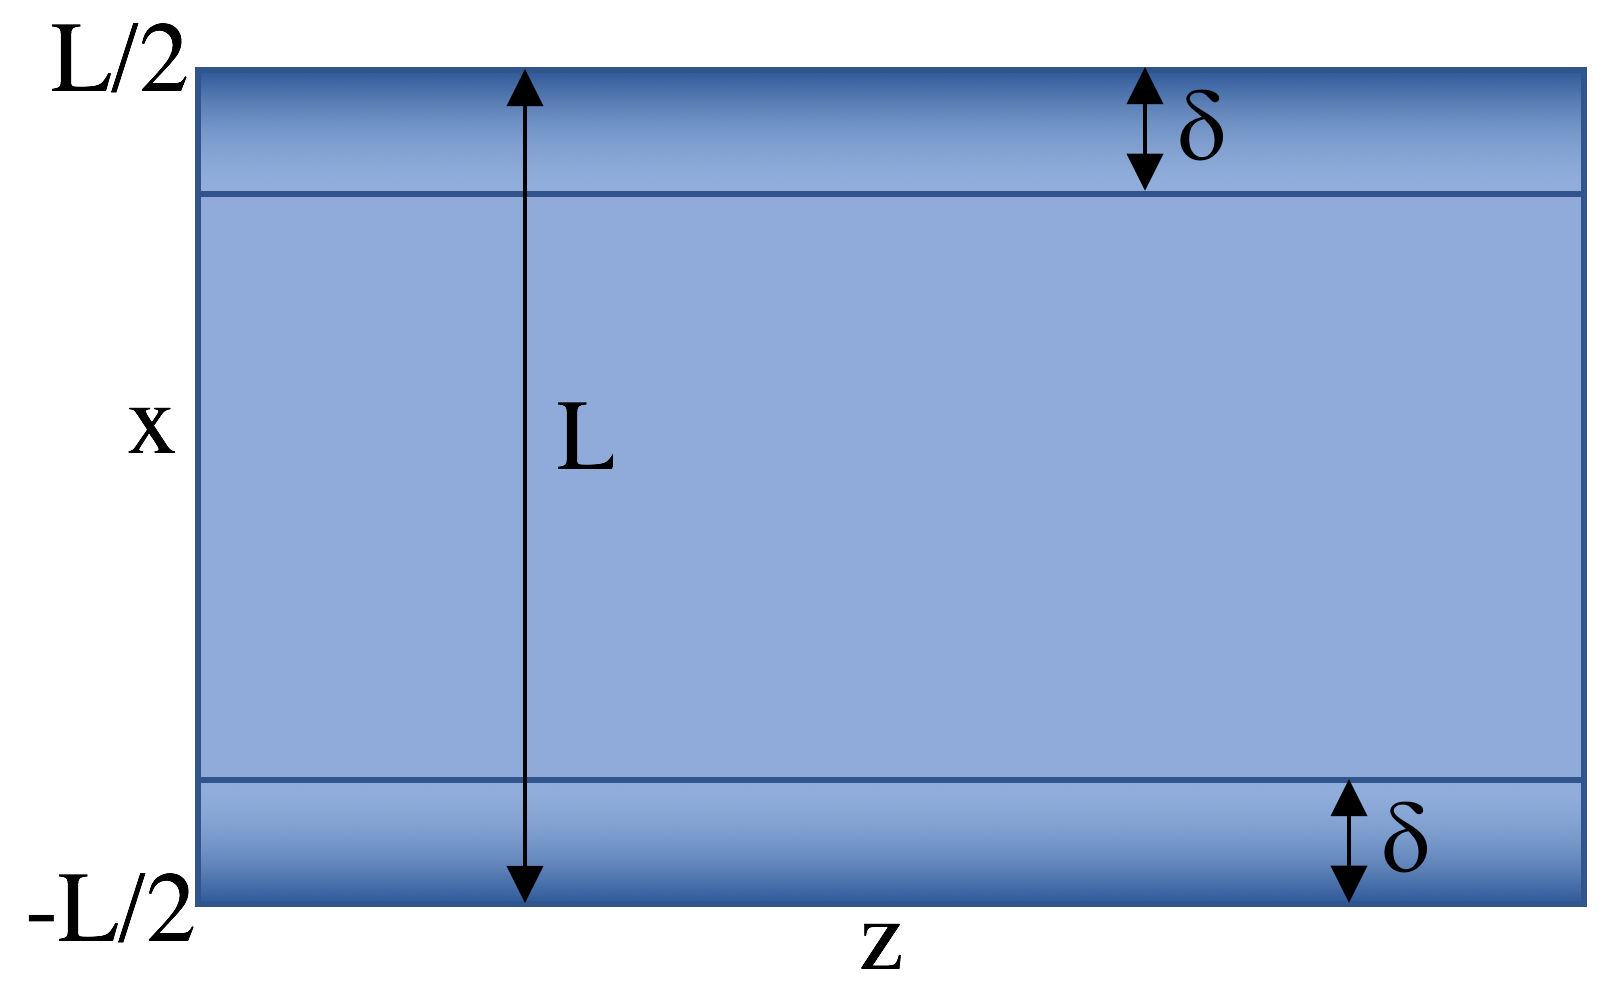
\includegraphics[width=0.5\textwidth]{sketchN1.png}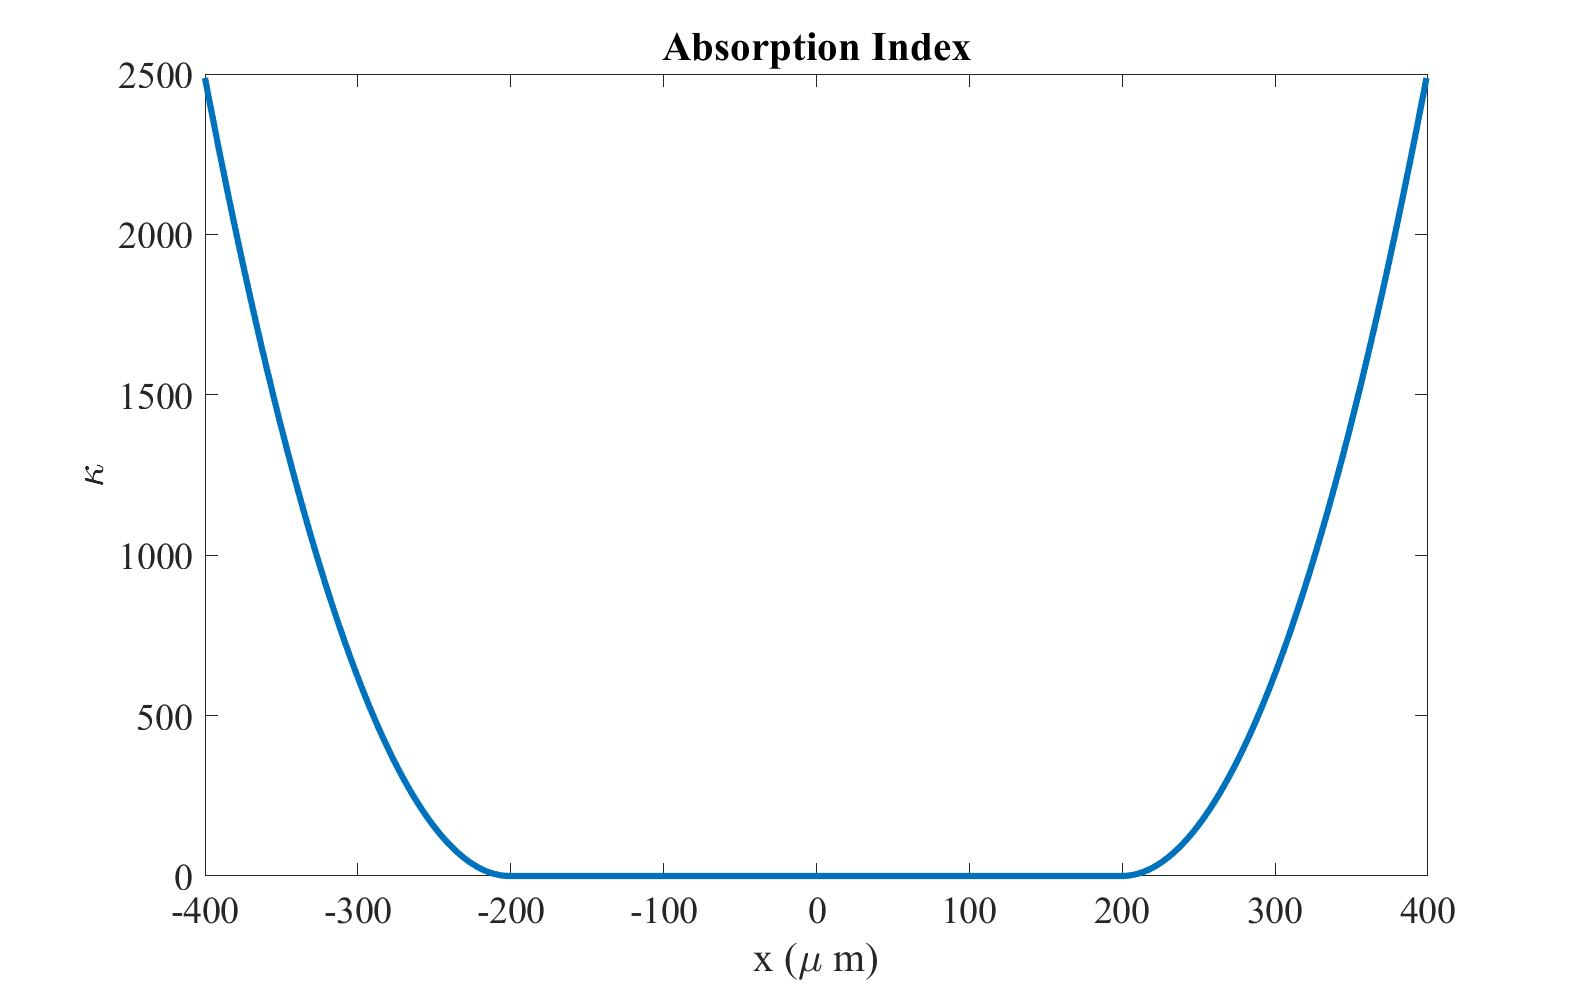
\includegraphics[width=0.5\textwidth]{N2.jpg}
		\caption{\label{fig:Absorption}Absorption boundary, figure on the right show the geometry of absorbed boundary, appropriate $\delta$ can be chosen during simulation time, figure on the left shows function absorption index $\kappa$ $ (x) $ and its change along x-direction.}
	\end{figure}
	\subsubsection{Error convergence}	
	In order to assess the accuracy of the numerical method, error is calculated. Error is a difference between numerical and analytical electric field and can be calculated using different norms. There is fixed relation between number of grid point and total error, if one increases the number of grid points, error is expected to decrease. If number of grid points is increased $2^n$ times, error should decrease $2^{-n}$ times, $n$ is integer number which also tells about order of error convergence.
	\[||Error||_2 = \frac{1}{\text{{\it Number of grid points}}}\sqrt{\sum\limits_{i=1}^n (E_{\text{\it z numerical}}-E_{\text{\it z analytic}})^2 }
	\]
	\[
	||Error||_\infty = (E_{\text{\it z numerical}}-E_{\text{\it z analytic}})_{maximum}
	\]
	\[ ||Error||_{\text{\it at particular point}} = \text{\it Error at any particular physical point is recorded}
	\]
	\newpage
	\section{Results}
	Numerical algorithm and analytical solution were both implemented and compared, results can be seen in Figure \ref{fig:Results}. In first row depicts Crank-Nicolson numerical method, second row shows analytical solution, first and second columns show real component of electric field and intensity of light consequently. Parameters of laser beam in our case are: z-meshsize = x-meshsize  = 1 $\mu m$, wavelength ($\lambda$) = 20 $\mu m$, waist ($w_o$) = 30 $\mu m$, refractive index ($n_o$) = 1.	
	\begin{figure}[h!]
		\hspace{-30mm}
		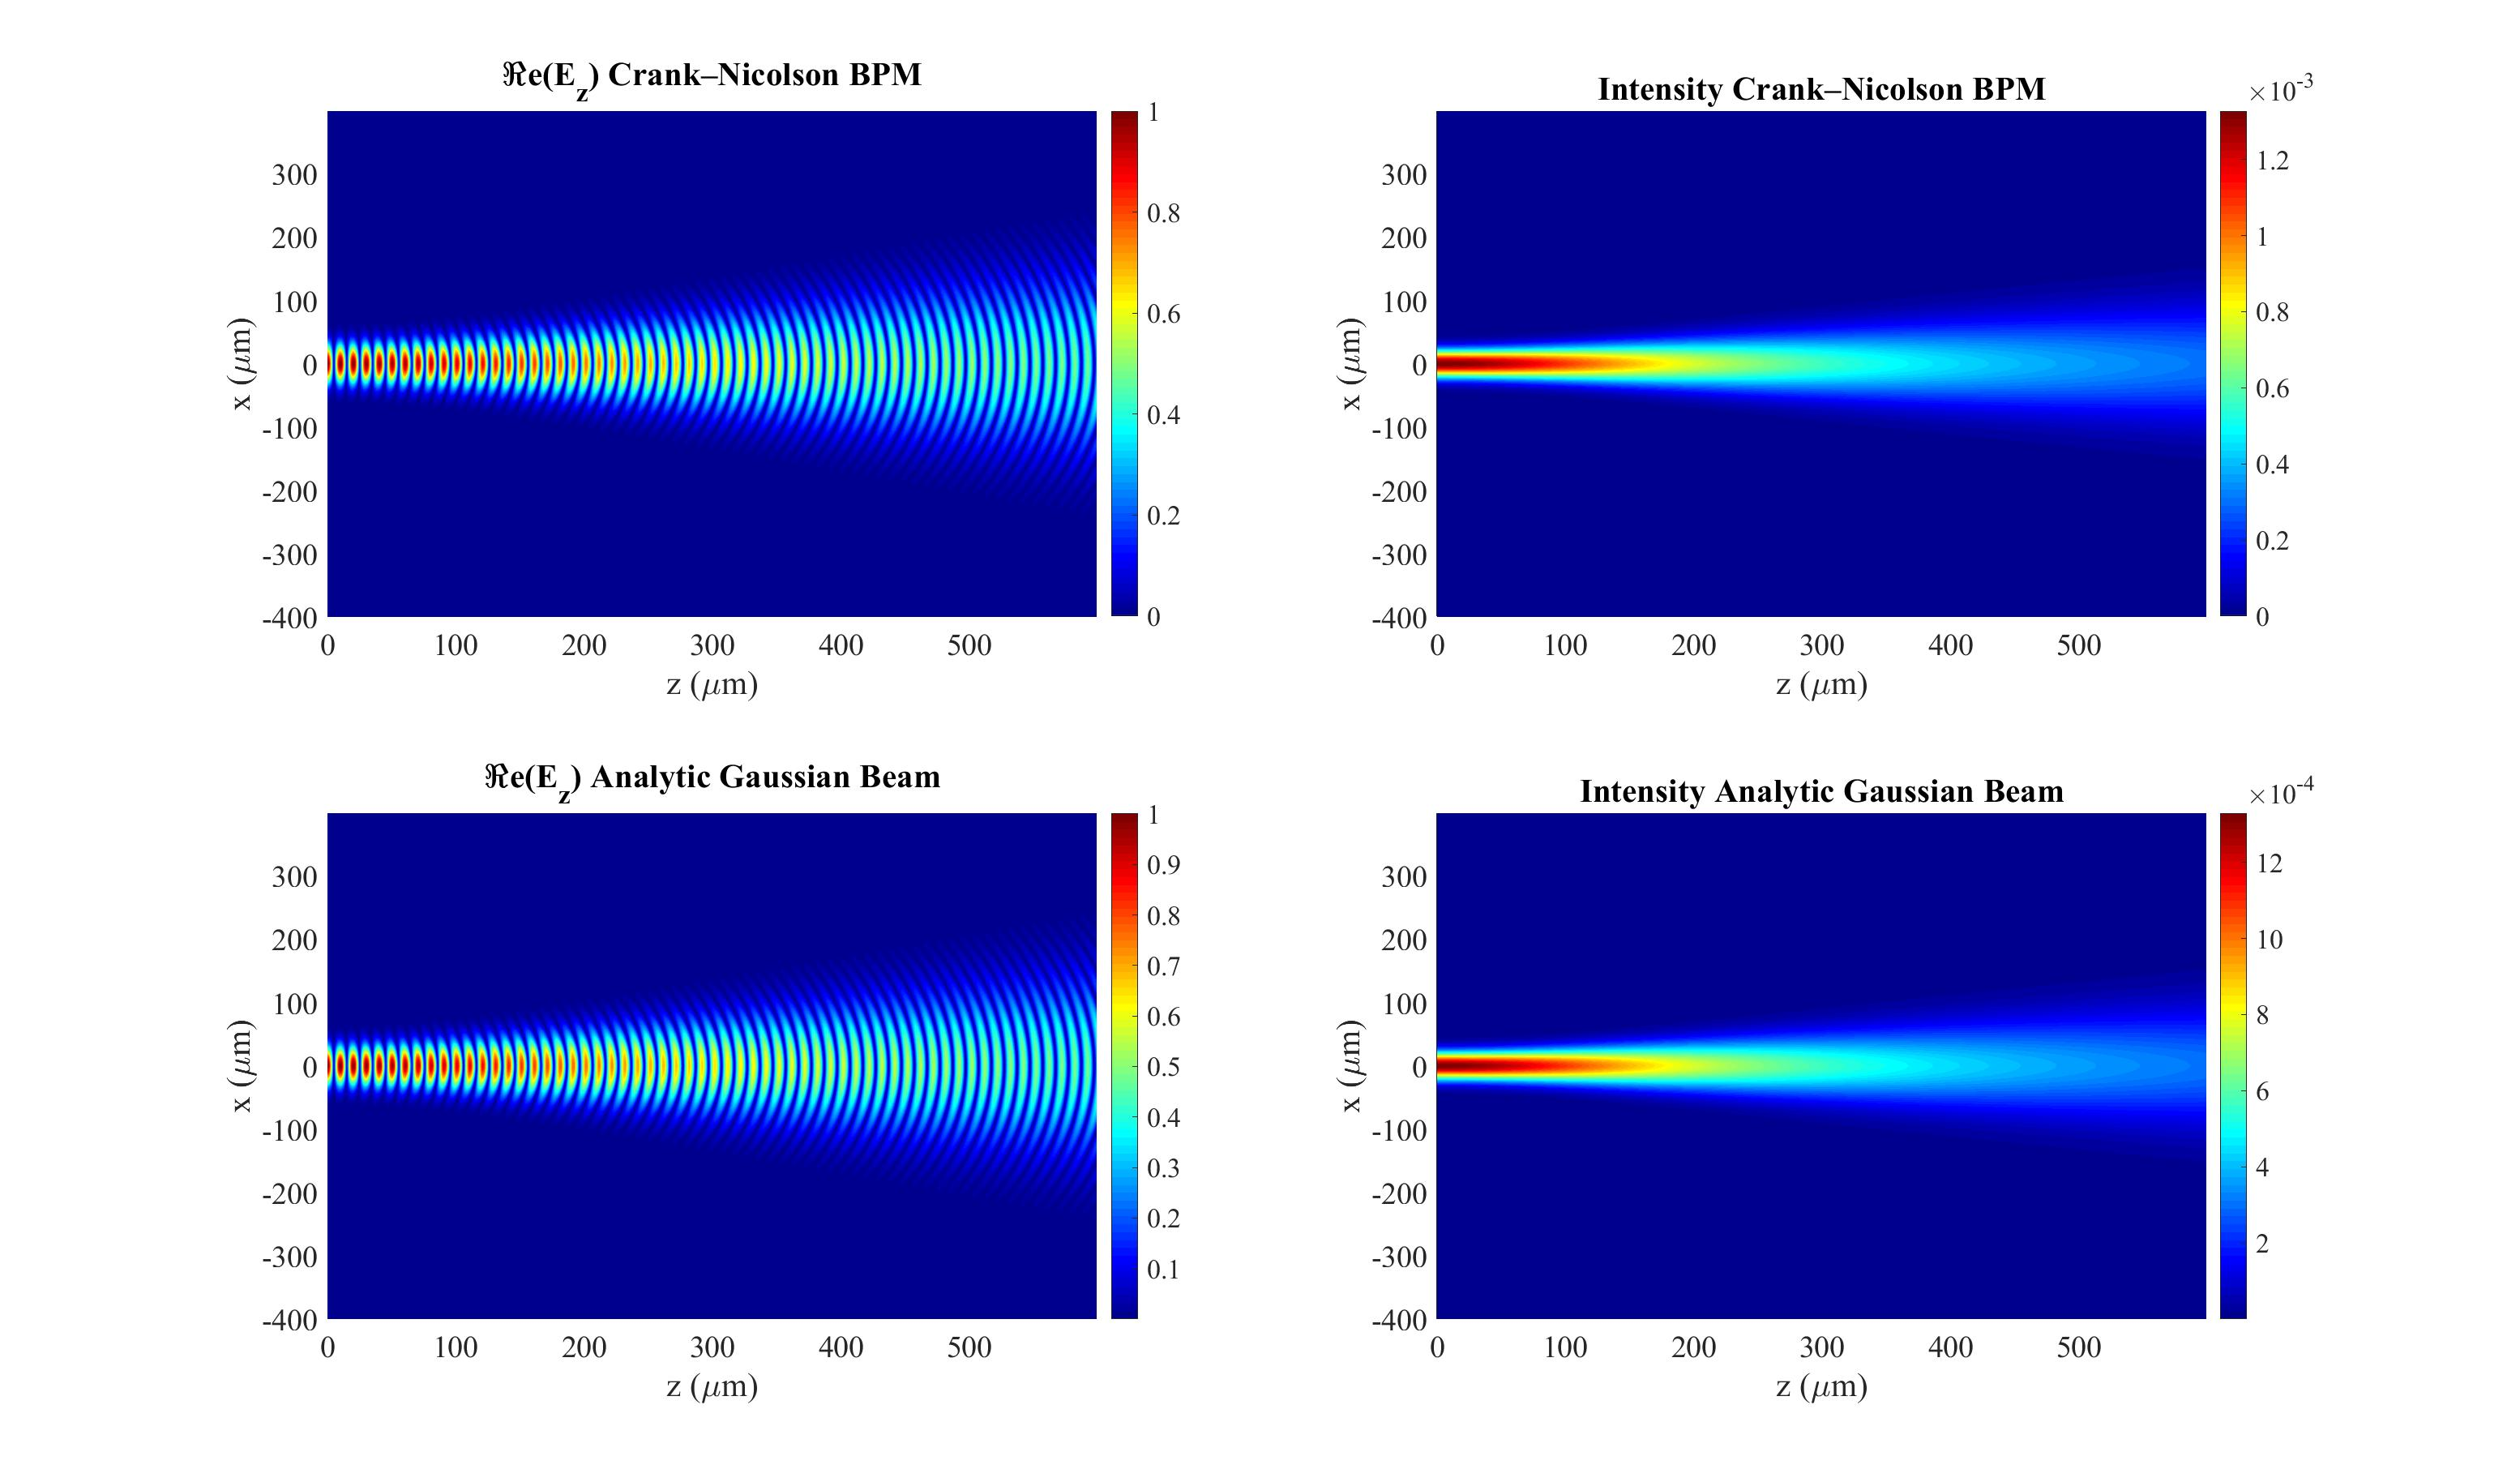
\includegraphics[width=1.5\textwidth]{N1.jpg}
		\caption{\label{fig:Results}Comparison of two methods.}
%		\centering
	\end{figure}
	\subsection{Absorption Boundary Condition}
	In this section we show the results of applying ABC. In Figure \ref{fig:Absorption2} the necessity of applying ABC can be seen.
	
	\begin{figure}[h!]
		\hspace{-30mm}
		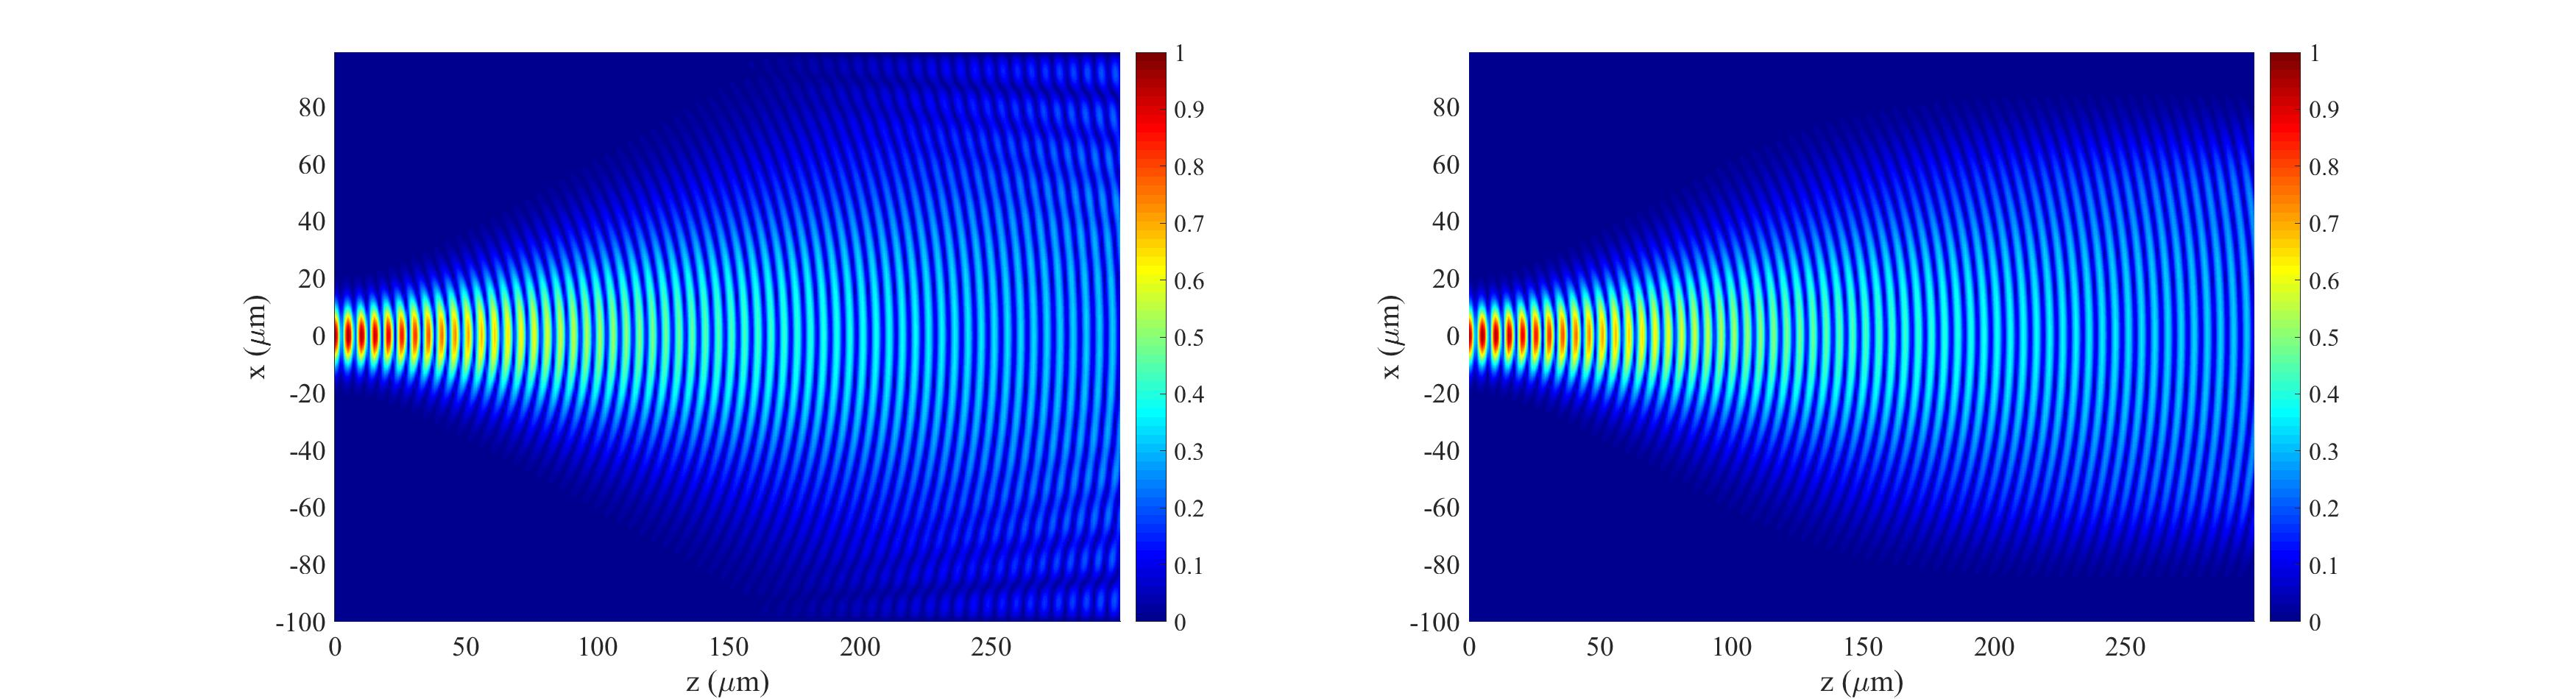
\includegraphics[width=1.5\textwidth]{N3.jpg}
		\caption{\label{fig:Absorption2}Comparison of two methods.}
%		\centering
	\end{figure}
	\newpage
	\section{Conlusion}
	\end{document}




